\section{Design and Implementation}
\label{sec:implement}

\NM{} is designed as a drop-in replacement for the default memory allocator. It intercepts all memory allocation/deallocation APIs via the preloading mechanism. Therefore, there is no need to change the source code of applications to employ \NM{}, and there is no need to use the custom OS or hardware. 

Different from existing work, \NA{} aims to reduce remote accesses, and balance the workload among different hardware nodes. It also utilizes huge page support to improve the performance, and designs its interleaved and block-wise memory allocation to accommodate shared objects. Multiple components that differentiate it from existing allocators are discussed in the remainder of this section. 
  
\NA{} also borrows many known mechanisms of existing allocators. First, it utilizes the size class to manage objects. Instead of allocating the exact size, \NA{} will round the size of an allocation to its closest size class. Similar to TcMalloc~\cite{tcmalloc}, \NA{} also utilizes fine-grained size classes for small objects, such as 16 bytes apart for objects less than 128 bytes, and 32 bytes apart for objects between 128 bytes and 256 bytes, then power-of-2 sizes afterwards. Second, it utilizes the ``\textbf{Bi}g-\textbf{B}ag-\textbf{o}f-\textbf{P}ages'' mechanism that all objects in the same page will have the same size class, and separates the metadata from actual objects. \NA{} only tracks the size information of each page, which helps reduce its memory overhead for the metadata. Third, \NA{} utilizes freelist to manage freed objects. Every freed object will be added into a corresponding freelist, and objects in the freelist will be allocated first in order to reduce possible cache misses. Further, \NA{} utilizes the first word of freed objects to link different objects, which is similar to Linux and TcMalloc~\cite{tcmalloc}. This mechanism helps to reduce the memory overhead, but is prone to memory vulnerabilities, such as buffer overflows and double-frees~\cite{DieHarder, Guarder}.     

\begin{figure*}[h]
\begin{center}
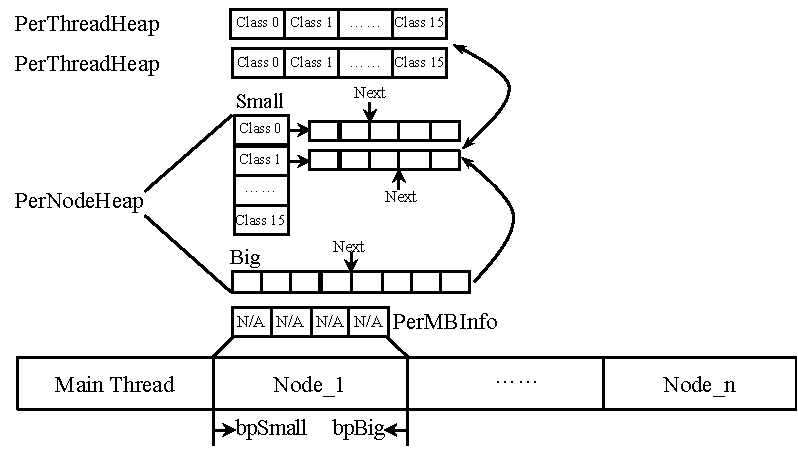
\includegraphics[width=0.8\textwidth]{figure/heaplayout}
%\includegraphics{figure/overview2}
\end{center}
\vspace{-0.1in}
\caption{Overview of \NA{}.
\label{fig:overview}}
\vspace{-0.1in}
\end{figure*}

\subsection{Topology Aware Task Assignment} 
\label{sec:taskassign}

Existing allocators typically do not schedule tasks explicitly, but relying on the default OS scheduler. The OS scheduler performs very well for the UMA architecture, since the latency of accessing the memory controller is the same for every core. However, the NUMA architecture imposes additional challenge~\cite{Majo:2015:LPC:2688500.2688509}. If a task is moved to a new node, it has to access all of its memory through the interconnect, resulting in a higher memory latency. The scheduling may lead to significant performance difference for memory-intensive applications. Therefore, typically tasks are bound to a specific core/processor for the NUMA architecture~\cite{terboven2012assessing, terboven2012task, Majo:2015:LPC:2688500.2688509}.  

%Similarly, \NA{} embeds the task assignment into its memory management. 
Due to the importance of task assignment to  memory locality, \textit{\NA{} embeds a topology-aware task assignment, which makes it different from existing allocators}. Every thread is bound to a specific node, where its memory allocations will be based on the location of its task, as described in Section~\ref{sec:nodeaware-memory}. \NA{} utilizes a round-robin manner to manage the tasks, which is similar to TBB-NUMA~\cite{Majo:2015:LPC:2688500.2688509}. This ensures that each processor/node will have a similar number of threads, and therefore a similar workload. 

In the implementation, \NA{} recognizes the hardware topology via the \texttt{numa\_node\_to\_cpus} API, which tells the relationship between each CPU core and each memory node. It intercepts all thread creations in order to bind a newly-created thread to a specific node. \NA{} employs \texttt{pthread\_attr\_setaffinity\_np} to set the attributes of a thread, and passes the attribute to its thread creation function. Therefore, every thread is scheduled to the specified node upon the creation time. Note that a thread is pinned to a node in \NM{}, instead of a core, which still allows the OS scheduler to perform the load balance when necessarily. 

\subsection{Node-Aware Memory Management} 
\label{sec:nodeaware-memory}

\NA{} designs a node-aware memory management based on its task assignment. All heap objects of a thread will be \textit{physically} allocated from the node that the thread is currently pinned to, unless otherwise stated (Section~\ref{sec:mainthread}). Since a memory allocator only deals with virtual memory, but not physical memory, \textit{\NA{} binds every range of its virtual memory to a particular node via the \texttt{mbind} system call}. Therefore, \NA{} is able to identify the physical node information based on a virtual address, which is the same as existing work~\cite{tcmallocnew}. However, \NA{} manages memory allocations and deallocations differently, which explains its significant performance advantage over the existing work~\cite{tcmallocnew} (see Section~\ref{}). 

%Since every thread has been bound to a particular node, without the migration, 
\NA{} handles deallocations of objects carefully, in order to prevent unnecessary remote accesses. \NA{} handles large objects and small objects differently. The assumption is that an application typically has a large number of small objects, but with relatively fewer number of big objects. Also, every big object has a larger impact on the memory consumption, which should be re-utilized as soon as possible. In \NM{}, freed objects with the size larger than 512KB will be always tracked in the per-node freelist, while \NA{} maintains per-node freelist and per-thread freelist for small objects. During each memory deallocation, \NA{} determines its physical node (based on its virtual address) and the size information of an object in order to place it correspondingly. A big object is always placed into a per-node freelist, while a small object will be based on its location information: if the object is allocated from a different node, it will be placed into the common freelist of that node; Otherwise, it will be placed into the per-thread freelist of the deallocation thread. The reason of utilizing per-thread list is that there is no need for the synchronization when accessing the per-thread list, since only one thread will access it, which helps the performance and scalability overall. \NM{} handles big objects differently with existing allocators that big objects are not returned to the OS immediately upon deallocations~\cite{Hoard, tcmalloc}. Further, big objects can be utilized to satisfy allocation requests of small objects, since the size of a big object is always multiple times of the bag size of small objects.  

 
\NA{} manages memory allocations as following. Basically, an allocation will be satisfied from the corresponding freelist at first, if some freed objects exist. Otherwise, a new/never-used object will be allocated. This design not only reduces possible memory consumption by avoiding the use of new memory, but also reduces possible cache misses since freed objects are likely to be hot in the cache. Objects in the same freelist will be allocated using the last-in-first-out order, which helps reduce possible cache misses since last-freed objects are more likely to be hot. As described above, a big object will be allocated from the per-node freelist, while a small object will be allocated from the thread's per-thread list if possible and then the per-node freelist. \NM{} moves objects between per-thread lists and per-node lists: if freed objects in a per-thread list is over a pre-defined threshold, a percentage of freed objects will be moved to per-node lists; Whenever the per-thread list is empty, some  objects will be moved from the corresponding per-node freelist. Both direction of movement will take an adaptive mechanism. For instance, if a per-thread list keeps move the objects from its per-node list, then the percentage of moving to per-node list will be reduced every time. Similarly, if a per-node list do not have objects to move to the per-thread list, \NM{} will check and move less frequently.  

 
 %If a memory request belongs to a large object,  
%There is no need to acquire the lock Allocations from its per-thread freelist, there is no lock to protect, which could reduce the synchronization overhead. For memory allocations, objects in a freelist will be used first before never-allocated objects, in order to reduce memory consumption and reduce possible cache misses.  
%Third, during the allocation, \NA{} will be always satisfied by objects in the freelist first. 

\NA{} reduces the overhead of frequent system calls, and borrows the information-computable design from existing allocators to quickly locate the physical node information~\cite{FreeGuard, Guarder}. The basic idea of its memory layout is illustrated in Figure~\ref{fig:overview}. Basically, \NA{} employs the huge address space of 64-bits machine to achieve the quick lookup. Instead of frequently allocating the memory from the OS, \NA{} obtains a big chunk of memory (few terabytes) from the underlying OS initially, and then divides it to multiple chunks with the same size. Each chunk will be bound to a specific memory node, as described in the above. Therefore, the physical node information could be computed  directly from the virtual address, by checking the distance from the starting address of the heap. Comparing the method of using a hash table to track the node information~\cite{tcmallocnew}, this mechanism is much faster since it avoids the  conflict that multiple ranges of addresses may locate in the same bucket. 

In the implementation, 
the size of each big object is always multiple Megabytes. For each deallocation of big objects, it will always concatenate with its neighbors to form a larger block if possible.       

\subsection{Interleaved and Blockwise Memory Allocation for Shared Objects} 
\label{sec:mainthread}

\NA{} designs a new interleaved and blockwise memory allocation for shared objects, which is different from all existing allocators. Based on our observation, most NUMA performances issues identified by existing NUMA profilers are related to shared objects~\cite{XULIU, MemProf}. Shared objects are typically allocated in the main thread, but are accessed concurrently by multiple children threads later. This may introduce load imbalance issue that the node  of the main thread may have much more memory accesses than other nodes, if multiple threads are accessing shared objects.   

In \NA{}, shared objects are allocated from a special range of memory where the physical memory will be allocated from all nodes interleavedly, via the \texttt{mbind} system call. This design helps balance the volume of memory accesses of all memory controllers, reducing interconnect congestion. Additionally, \NA{} also allocates the memory in a block-wise way, when the size of an allocation is multiple times of the page size. That is, each block will be equal to the division of the size of an allocation by the number of threads. The block-wise allocation helps to reduce remote accesses, if every thread is accessing a block of memory continuously. 
 
During the implementation, \NA{} proposes to identify shared objects with the allocation/deallocation pattern based on the allocation callsite. \NA{} assumes that objects from the same callsite will have the same shared pattern, since that depends on the program logic. \NA{} monitors allocations and deallocations: if a newly-allocated object has been deallocated in the main thread before creating children threads, then this object cannot be shared by multiple threads and its corresponding callsite is considered to be a private callsite. Otherwise, it is considered to be a shared callsite and all objects from this callsite will be allocated  from a special range that will be allocated interleavedly among all memory nodes. 

\NA{} utilizes the sum of stack position (e.g., size parameter) and the return address to identify a callsite. When memory allocations are invoked in different functions, their stack positions are likely to be different. The return address (of the application) typically tells the different placement inside the same function. This design  avoids the mis-identification issue of using one level of callstack, when there exists allocation wrappers. \NA{} is also meticulously implemented to avoid the performance issue. It obtains the return address quickly via an offset. The stack placement with this offset stores the return address of the allocation callsite. We do not utilize the slow \texttt{backtrace} function, and do not use the built-in function (e.g, \texttt{\_\_builtin\_frame\_address}) that can be omitted by the compiler in some optimization levels like \texttt{-O2}.  


\NA{} utilizes a hash table to track the status of every callsite. Upon every allocation, \NA{} will check the status of the allocation callsite, with the key to be the sum of stack position and the return address. If the callsite is shared, then the current allocation will be satisfied from the interleaved heap. For each deallocation, \NA{} checks whether the corresponding allocation is allocated from the same epoch. If that is the case, then the corresponding allocation callsite will be marked as  private. 

% However, this policy may cause multiple performance issues. First, it may cause load imbalance issue where the initial node have much more accesses than other nodes. Second, it may lead to a large number of remote accesses, since children threads may not run in the same node as the main thread. To address such issues, \NA{} proposes to identify shared objects with the allocation/deallocation pattern, and then infers the OS to allocate physical memory in an interleaved and blockwise way. Therefore,  \NA{} monitors the allocation and deallocation pattern for heap objects. If a calllsite is considered to have shared objects, 
  
%If an object is not shared between multiple threads, most existing allocators will allocate such objects from the local node, causing no performance issue.   the main thread typically prepares the data for all of its children threads. That is, it is very likely that most objects allocated from the main thread will be shared by most threads. Therefore, it will cause the load imbalance issue, if all objects from the main thread are allocated from the node that the main thread is running on. Also, it could also introduce significant number of remote accesses, since not all threads could run on the same node.  

%\paragraph{Children Threads:} For normal threads, it is better to allocate the memory from the local node, in order to reduce remote accesses. But existing allocators have an issue to handle remote frees that the deallocation thread is not the same as the allocation thread~\cite{Aigner:2015:FML:2814270.2814294}. They tend to place freed objects into the current thread, such as TCMalloc~\cite{tcmalloc} or jemalloc~\cite{jemalloc}, no matter where these objects are allocated from.  However, this could cause remote accesses. In order to solve this issue, \NM{} proposes an information-computable design, as shown in Figure~\ref{fig:overview}. Basically, \NM{} utilizes the fact of 64-bit address space, where machines have extremely large amount of virtual address. Basically, \NM{} requests 32 TB virtual address at one time, and then divides it to multiple spans based on the number of nodes. For each span, \NM{} binds the memory to a specific node through \texttt{mbind} system call. Therefore, \NM{} is able to recognize the physical location by the address. During the deallocation, \NM{} will actually return a remote object to its owner, and only return the objects from the current node to the current thread's PerThreadHeap. 


\subsection{Automatic Huge Page Support} 

\NA{} utilizes the huge page support to further improve the performance. Modern hardware typically installs with huge page support. A huge page is a page that its page size is much larger than 4 kilobytes. Currently, the Linux system has two page sizes, 4 Kilobytes and 2 Megabytes. Based on the existing study~\cite{hugepages}, huge pages can reduce Translation Look-aside Buffer (TLB) misses that may significantly affect the performance in multi-level page table. A TLB entry will cover a larger range of memory, which will need less TLB entries to cover the working set of an application. Reducing the TLB misses also reduces the interference on the cache utilization caused by TLB misses. We observed around 10\% performance improvement for some applications, when we are using huge page support. 

However,  

The default huge page support is not good for the performance~\cite{}. It also may have some harmful impact on the performance. However, if the huge page is utilized very well, the application's performance can be improved dramatically. To taking advantage of this benefit, each PerNodeHeap is further divided into two parts, where small objects will be allocated from the beginning and will be allocated using small pages, while big objects will be allocated from the end of the heap using huge page (2MB). We believe that this mechanism balances the performance and memory consumption.   

We don't use huge pages for small objects, in order to avoid possible false sharing issue. 


\subsection{Reutilization of Big Objects} 
Existing allocators will handle big objects different with small objects, which will be allocated from the OS directly. When these objects are freed, they will be returned to the OS directly by invoking \texttt{munmap} or \texttt{madvise}. This mechanism was designed to reduce memory consumption. However, this mechanism will invoke a lot of unnecessary overhead, since a big object may include numerous pages and cache lines.  Returning big objects to the OS may require to reload these pages and cache lines if an application actually requires more memory.  
%Taking an object with the size of 1 MB as the example, this object includes 256 pages (4KB). Therefore, the overhead includes returning 256 pages to the OS (by modifying the page table entries of 256 pages), and then 256 page faults when this is returned. 
%More importantly, cache lines of these 256 pages should be reloaded from the memory after allocating these physical pages. 
%\NM{} aims to reduce such overhead based on a simple assumption: if the application is requesting memory, then big objects should not be returned to the OS to avoid such overhead. In fact, 
\NM{} proposes to utilize these big objects for small objects, instead of returning them back to the OS. Due to this design, \NM{} actually utilizes 1MB as the basic unit, and then allocates 1MB for small objects on demand. 

\subsection{Other Improvements:}

\paragraph{Node-local Metadata:} \NM{} designs the metadata meticulously, which will be always allocated in the same node. Such metadata includes the PerMBInfo, freelists for different size classes, and freelists for big objects. PerThreadHeap's metadata will be also allocated in the local node as well, which has been assigned to a specific node during thread creation. 


\subsection{Node-Local Allocation}

What is the basic idea of allocation? 
Basically, upon receiving a request, \NM{} will check the size of the object at first. If the size is less than the threshold of big objects, this is a small object. 

For small objects, \NM{} will always allocate them from the PerThreadHeap. Since a PerThreadHeap will be only utilized by one thread, it won't need the synchronization, and possibly has the better scalability. 

\subsection{Special Support for Main Thread}
\NM{} provides the special support for the main thread, which is motivated by a lot of existing tools ~\cite{XULIU, MemProf}. Based on their paper, many of NUMA related performance problems are caused by one type of objects that were allocated in the main thread but shared by multiple children threads. To prevent these issues, they proposed to change the code explicitly, using a group of threads that were bound to different nodes to perform the initialization. However, these changes are not automated, which should also rely on the test results of these NUMA tools.  

%nstead, \NM{} proposes an automatic method to deal with these issues. Due to the fact that many objects will be shared by children threads later, \NM{} allocates objects from the main thread in a separate heap, which mainly focuses on the load imbalance. To achieve the load balance, one simple technique is to allocate objects that will be physically allocated with an interleaved way. However, this simple technique does not work due to the following reasons. 

%First, not all objects are shared by multiple threads. Some objects will be just accessed by the main thread. For these objects, if their corresponding physical pages are allocated in remote nodes, they could  incur remote accesses unnecessarily. Therefore, \NM{} should avoid unnecessary remote accesses by recognizing which objects are private objects, and allocating these objects locally.  

%Second, load balance alone cannot guarantee the optimal performance, if objects are accessed block-wise by multiple threads. In fact, this is more common based on existing studies~\cite{XULIU, MemProf}. \NM{} supports block-wise memory allocation for big objects.  

%Third, the allocation should take advantage of huge pages that is already available in most existing hardware. \NM{} takes this into account for its design and implementation. In fact, \NM{} divides the memory into three spans. 

%Fourth, big objects will utilize a lot of memory, which should be handled carefully. We can't reutilize these objects for node-local allocations, which may incur unnecessary remote accesses. Also, we don't want to waste the physical memory for these objects. Instead, \NM{}  will return these objects to the OS directly during the deallocation. 

%During the implementation, \NM{} should detect private objects. It utilizes a simple rule to detect private objects: if an object is deallocated in the main thread before the creation of children threads, then this object is not shared by other threads. However, if an object has been allocated in the special heap, it cannot be changed easily with a low overhead. We further propose a call-site based mechanism: objects from the same callsite will typically have the same deallocation behavior. Objects will be allocated in the special heap at first, but will be allocated in the normal heap if some objects from the call callsite were identified as private objects. \NM{} therefore maintains two hashmap to track such objects: one hashmap is used to track private callsite, and another hashmap is used to track the relationship between objects and their corresponding callsites. During the allocation, \NM{} will check whether the callsite is private or not. If the corresponding callsite has been identified as the shared one, then it will be allocated from the special heap. If the corresponding callsite has not been tracked before, then this object will be allocated form the special heap, and the corresponding object will be placed in the hashmap that tracks the relationship between objects and their corresponding callsites. 


%For private objects, its deallocation phase is the same as the allocation phase. Therefore, we will track the phase information there. 
%We will use the phase 0 to indicate that the phase is not in the main thread phase. Otherwise, we will use the number to indicate it.   

\subsection{Huge Page Support}

 
Huge page could reduce the TLB misses, and further reduce the cache pollution caused by TLB misses. However, 
However, it is 



%https://queue.acm.org/detail.cfm?id=2852078

